\documentclass[11pt,a4paper]{article}

\usepackage[margin=2.2cm]{geometry}
\usepackage[T1]{fontenc}
\usepackage[utf8]{inputenc}
\usepackage{lmodern}
\usepackage{microtype}
\usepackage{xcolor}
\usepackage{hyperref}
\usepackage{booktabs}
\usepackage{longtable}
\usepackage{array}
\usepackage{listings}
\usepackage{tikz}
\usetikzlibrary{positioning}
\usepackage{enumitem}
\usepackage{fancyhdr}

\hypersetup{
  colorlinks=true,
  linkcolor=blue!50!black,
  urlcolor=blue!50!black,
  pdftitle={Assignment 2 Experiment Tracking Notes}
}

\pagestyle{fancy}
\setlength{\headheight}{14pt}
\fancyhf{}
\lhead{Assignment 2 Tracking Notes}
\rhead{\thepage}

\definecolor{codebg}{RGB}{245,245,245}
\definecolor{codeframe}{RGB}{220,220,220}
\definecolor{codekw}{RGB}{0,70,140}
\definecolor{codecomment}{RGB}{0,120,60}
\definecolor{codestring}{RGB}{160,60,0}

\lstdefinestyle{mystyle}{
  backgroundcolor=\color{codebg},
  frame=single,
  rulecolor=\color{codeframe},
  basicstyle=\ttfamily\small,
  keywordstyle=\color{codekw}\bfseries,
  commentstyle=\color{codecomment},
  stringstyle=\color{codestring},
  showstringspaces=false,
  breaklines=true,
  columns=fullflexible
}

\lstset{style=mystyle}

\title{Assignment 2\\Experiment Tracking Notes}
\author{Working document for benchmarking and report planning}
\date{May 5, 2026}

\begin{document}

\maketitle

\section{Purpose}

This document is a working LaTeX note for tracking experiment ideas, benchmark plans, implementation decisions, and report-ready observations for the Irish-to-English speech translation assignment.

\section{Confirmed Evaluation Setup}

\begin{itemize}[leftmargin=1.4em]
  \item Evaluation split: \texttt{iwslt2023\_ga-eng/dev}
  \item Reason: \texttt{iwslt2026\_ga-eng/test-2026} is a blind test set and does not contain English reference translations.
  \item Report requirement: clearly document the split used and the exact data source, including the linked submodule.
\end{itemize}

\section{Current Dataset Notes}

\begin{itemize}[leftmargin=1.4em]
  \item Available locally:
  \begin{itemize}[leftmargin=1.6em]
    \item audio files in \texttt{dev/wav}
    \item English references in \texttt{dev/txt/dev.eng}
    \item metadata in \texttt{dev/stamped.tsv}
  \end{itemize}
  \item Important limitation:
  \begin{itemize}[leftmargin=1.6em]
    \item no plain gold Irish transcript file was identified in this local copy
    \item BLEU and chrF++ can be computed for English translation output
    \item standard transcript-to-transcript ASR evaluation against gold Irish text is not directly available from these files
  \end{itemize}
\end{itemize}

\section{Baseline Plan}

\begin{longtable}{>{\raggedright\arraybackslash}p{0.24\textwidth} >{\raggedright\arraybackslash}p{0.68\textwidth}}
\toprule
Component & Choice \\
\midrule
ASR & \texttt{openai/whisper-small} \\
MT & \texttt{facebook/nllb-200-distilled-600M} \\
Pipeline & audio $\rightarrow$ ASR transcript $\rightarrow$ MT English translation \\
Metrics & BLEU, chrF++, coverage, repetition rate \\
\bottomrule
\end{longtable}

\section{Why A Weak Baseline Is Still Useful}

\begin{itemize}[leftmargin=1.4em]
  \item A weak baseline does not ruin the assignment.
  \item It provides useful material for error analysis and discussion.
  \item It helps motivate the improvement section.
  \item It lets us study error propagation from ASR to MT.
\end{itemize}

\section{Planned Benchmark Experiments}

\subsection{Experiment 1: Baseline}

\begin{itemize}[leftmargin=1.4em]
  \item ASR: \texttt{whisper-small}
  \item MT: \texttt{nllb-200-distilled-600M}
  \item Goal: establish a standard cascaded baseline
\end{itemize}

\subsection{Experiment 2: Better ASR}

\begin{itemize}[leftmargin=1.4em]
  \item Replace \texttt{whisper-small} with \texttt{whisper-medium}
  \item Keep the MT model fixed
  \item Goal: isolate the effect of better ASR quality
\end{itemize}

\subsection{Experiment 3: Better MT}

\begin{itemize}[leftmargin=1.4em]
  \item Keep the baseline ASR
  \item Replace NLLB with another feasible GA$\rightarrow$EN translation model
  \item Goal: isolate the effect of MT quality
\end{itemize}

\subsection{Experiment 4: Direct Speech Translation}

\begin{itemize}[leftmargin=1.4em]
  \item Try a direct speech-to-English translation model if feasible
  \item Goal: compare cascaded ASR$\rightarrow$MT against end-to-end speech translation
\end{itemize}

\section{Suggested Evaluation Strategy}

\begin{enumerate}[leftmargin=1.6em]
  \item Debug each system on 50 examples.
  \item Run the most stable systems on a larger subset.
  \item If runtime is manageable, evaluate on the full dev split.
  \item Always compare systems on the same subset in the benchmark table.
\end{enumerate}

\section{Metrics To Report}

\begin{itemize}[leftmargin=1.4em]
  \item BLEU
  \item chrF++
  \item Coverage
  \item Repetition rate
\end{itemize}

\section{Error Analysis Checklist}

\begin{itemize}[leftmargin=1.4em]
  \item ASR substitution
  \item ASR deletion
  \item ASR hallucination
  \item MT untranslated tokens
  \item MT mistranslation
  \item MT over-generation
  \item Error propagation from ASR into MT
\end{itemize}

\section{Implementation Notes}

\subsection{Notebook Variables}

\begin{lstlisting}[language=Python, caption={Current dataset path setup}]
DATA_ROOT = Path("iwslt2023_ga-eng")
DEV_ROOT = DATA_ROOT / "dev"
AUDIO_DIR = DEV_ROOT / "wav"
TRANS_FILE = DEV_ROOT / "stamped.tsv"
REF_FILE = DEV_ROOT / "txt" / "dev.eng"
\end{lstlisting}

\subsection{Current ASR Note}

Whisper was tested as the baseline ASR model. In this setup, explicit Irish forcing with \texttt{language='ga'} was not available for the chosen Whisper model variant, so this limitation should be documented in the report.

\section{Benchmark Table Template}

\begin{longtable}{>{\raggedright\arraybackslash}p{0.34\textwidth}cccc}
\toprule
System & BLEU & chrF++ & Coverage & Rep. Rate \\
\midrule
Baseline: Whisper-small + NLLB-600M & -- & -- & -- & -- \\
Improved ASR: Whisper-medium + NLLB-600M & -- & -- & -- & -- \\
Improved MT: Whisper-small + Alternative MT & -- & -- & -- & -- \\
Direct ST model & -- & -- & -- & -- \\
\bottomrule
\end{longtable}

\section{Diagram Area}

This section can be expanded later with architecture diagrams or workflow figures.

\begin{center}
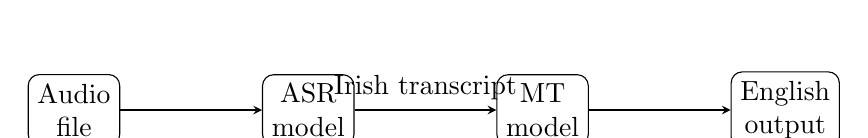
\begin{tikzpicture}[node distance=1.8cm, >=stealth]
  \node[draw, rounded corners, align=center] (audio) {Audio\\file};
  \node[draw, rounded corners, right=of audio, align=center] (asr) {ASR\\model};
  \node[draw, rounded corners, right=of asr, align=center] (mt) {MT\\model};
  \node[draw, rounded corners, right=of mt, align=center] (out) {English\\output};

  \draw[->] (audio) -- (asr);
  \draw[->] (asr) -- node[above] {Irish transcript} (mt);
  \draw[->] (mt) -- (out);
\end{tikzpicture}
\end{center}

\section{Code Snippet Area}

Use this area later to store code excerpts worth reusing in the report.

\begin{lstlisting}[language=Python, caption={Placeholder for future code excerpt}]
def placeholder():
    pass
\end{lstlisting}

\section{Report Framing Ideas}

\begin{itemize}[leftmargin=1.4em]
  \item Improving ASR should reduce downstream translation errors.
  \item Better MT cannot fully recover from a poor transcript.
  \item Direct speech translation may avoid some cascade errors, but may also be less robust depending on the model and language coverage.
  \item Any limitation around Irish language support must be reported clearly.
\end{itemize}

\section{Next Steps}

\begin{enumerate}[leftmargin=1.6em]
  \item Finalize the baseline pipeline.
  \item Compute baseline metrics.
  \item Inspect outputs manually.
  \item Compare at least one improved ASR system.
  \item Compare at least one improved MT system if feasible.
  \item If time allows, try a direct speech translation model.
\end{enumerate}

\end{document}
